\chapter{Machine Learning and Cybersecurity}\label{ch:machine-learning-and-cybersecurity}

Whether we realize it or not, our lifes have been uploaded.
This causes accumulation of big data, which are being used as training sets for Machine Learning methods and technologies such as image recognition, voice recognition and natural language processing.
The AI companies are spreading their products to all possible industries including transportation, healthcare or manufacturing.
Advancements in ML technologies are made possible by new dedicated hardware - CPU clusters, GPUs and Tensor Processing Units (TPUs), as well as software frameworks and platforms - TensorFlow, Microsoft's Computational Network ToolKit, Keras or scikit-learn.

% TODO: write a little bit more about how AI is a severe security risk, but on the other hand can be used for protecting our data, computers, etc.

\section{AI as a~tool for security breaches mitigation}\label{sec:ai-as-a-tool-for-security-breaches-mitigation}

The current generation of security products are incorporating ML technologies.
By training cybersecurity solutions on large datasets of network logs and suspicious files, the protection software aims to detect and block abnormal behavior, even if application or dataflow does not exhibit a~known malicious signature or pattern~\cite{blog:protocol_ai}.
In addition, those solutions can significantly reduce the amount of time needed for detection and response to malicious event.
Shortening the discovery times is critical - it takes about 206 days to spot a~breach and another 55 days to mitigate caused damage~\cite{blog:attack_detection_time}.
During that 206-day period, the threat could be performing a~range of malicious activities such as stealing sensitive corporate data or confidential information about customers.
ML helps security professionals to analyze security alerts in order to identify patterns that may indicate a~threat which could be missed otherwise.
Without help of AI supported systems, the IT department employees may not use their time efficiently - researching \textit{false positives} and \textit{dead ends}, while missing serious malicious activity.

Nowadays, people spend most of their time on a~computer or mobile phone by browsing.
If the hacker wants to infect a~device, the logical starting point is to create a~malicious website or compromise an existing one to carry out the task.
The attackers learned how to do URL injections (embeding malicious URLs or entire pages, through the victim page) or malicious redirects to a~page usually infected with malware or phishing forms.
Furthemore, malware uses for communication and URL leading to a~remote control server.
All this malicious activity in the system can be prevented by scanning traffic and analyzing network data.
Therefore a~fast URL classification systems which will automatically block all potential malicious activity of this type is really important.
In the chapter~\ref{ch:malicious-url-detection-and-classification} we will train such system.

\subsection{Fast retraining of models}\label{subsec:fast-retraining-of-models}

Training of ML model has been, for a~long time, the most lengthy and cumbersome part.
The frequency and size of the updates to ML models is increassing in order to keep up with offensive attempts - calling out for new techniques to ensure the engine being in accordance with the latest standards and to guarantee security of users.
\textit{Avira Operations GmbH} presents parallel training architecture.
The first training branch takes around 8 hours to complete.
In order to be able to quickly react to new threats, a~continuous retraining is performed every 15 minutes~\cite{whitepaper:avira_nightvision}.

\begin{figure}[htb]
    \centering
    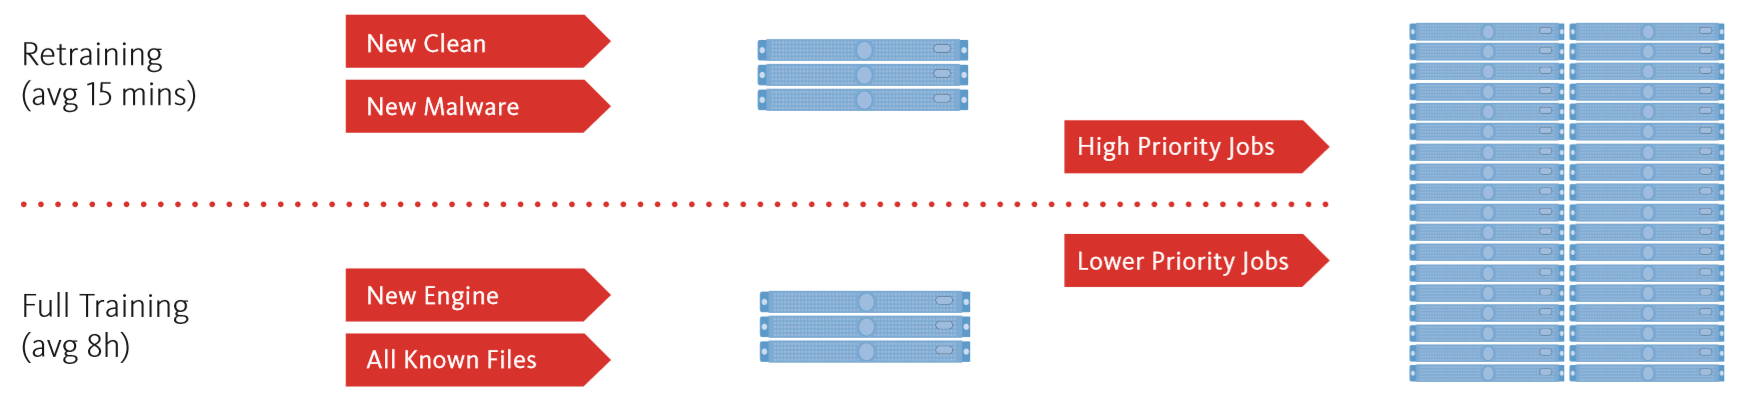
\includegraphics[width=0.9\textwidth]{imgs/avira_training.png}
    \caption{Avira's solution to keep security models up-to-date~\cite{whitepaper:avira_nightvision}}
    \label{fig:avira_training}
\end{figure}
\FloatBarrier

This rapid retraining approach is reducing the vulnerability that potentially exists with systems that are retrained daily or weekly~\cite{whitepaper:avira_nightvision}.

\subsection{Ransomware file detection}\label{subsec:ransomware-file-detection}

Different ML approaches can be used for different security objectives.
In white paper introduced by \crowdstrike, company providing cloud-native protection platform for enterprises, they present a~robust solution for ransomware detection.
By extraction of approximately one hundred features from files and their visualisations (e.g.\ file size, file entropy, number of sections, distribution of section entropy, imported \acrfull{dll} names, resource data, embedded \acrshort{ips}/domains, digital signature, etc.) is \crowdstrike able to train ML model for ransomware file classification~\cite{crowdstrike_machine_learning}.

\begin{figure}[htb]
    \begin{subfigure}{0.45\textwidth}
        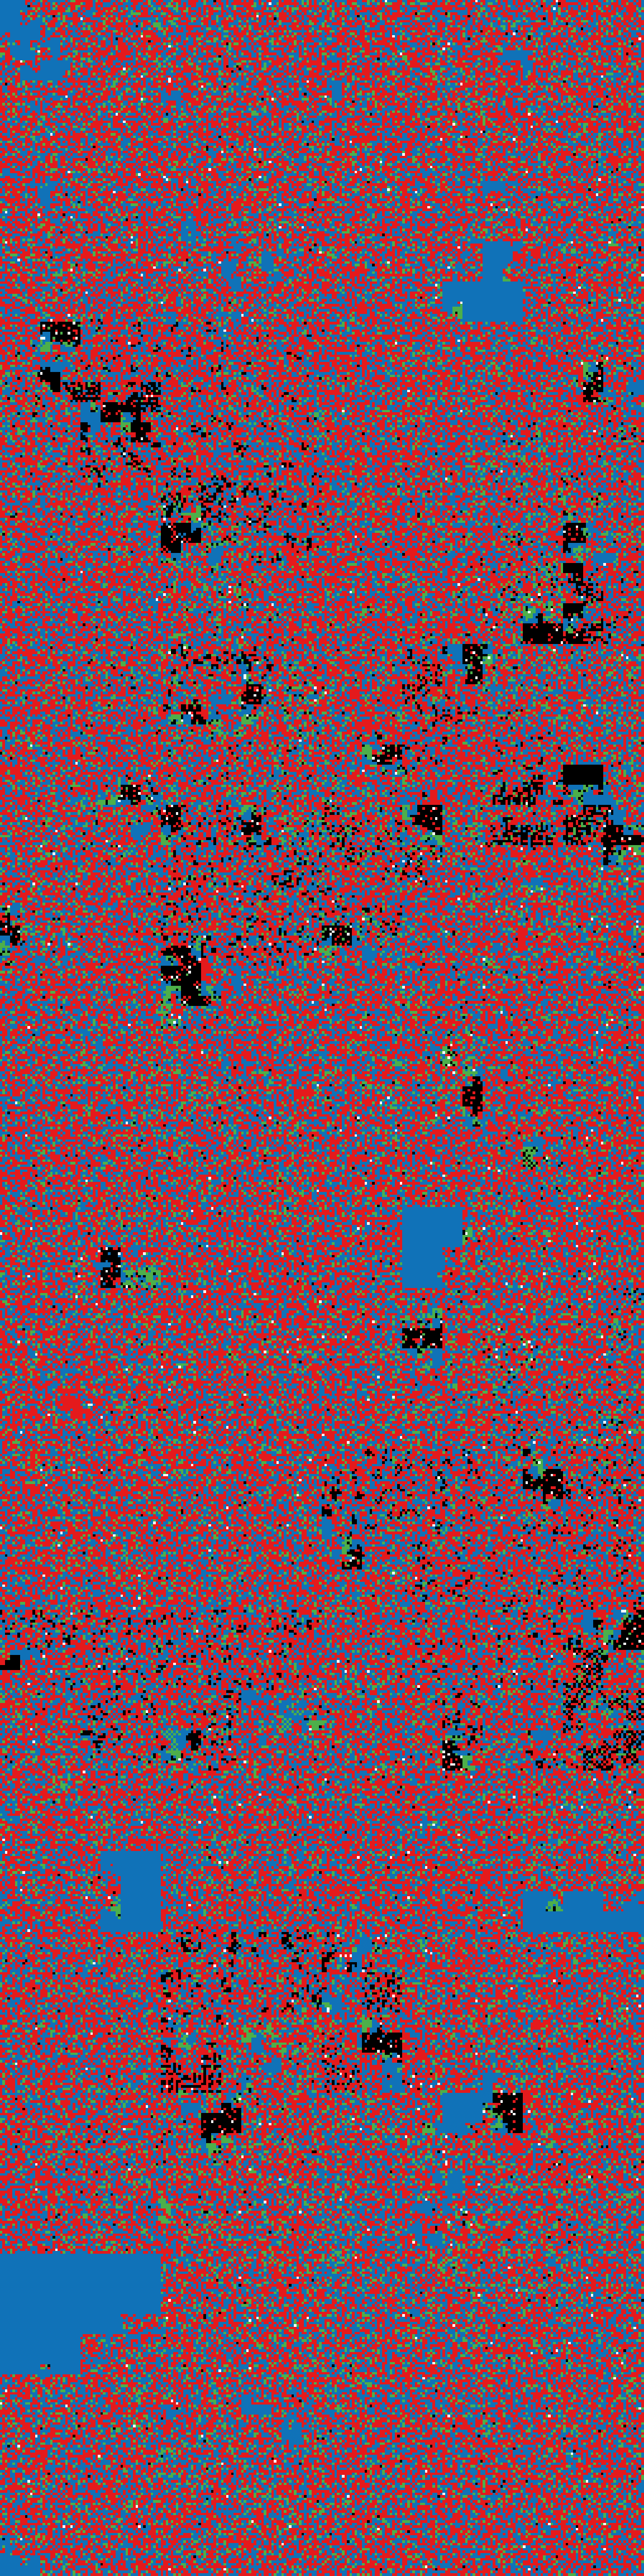
\includegraphics[height=5cm]{imgs/crowdstrike2.png}
        \centering
        \caption{file visualisation}
        \label{fig:subim1}
    \end{subfigure}
    \begin{subfigure}{0.45\textwidth}
        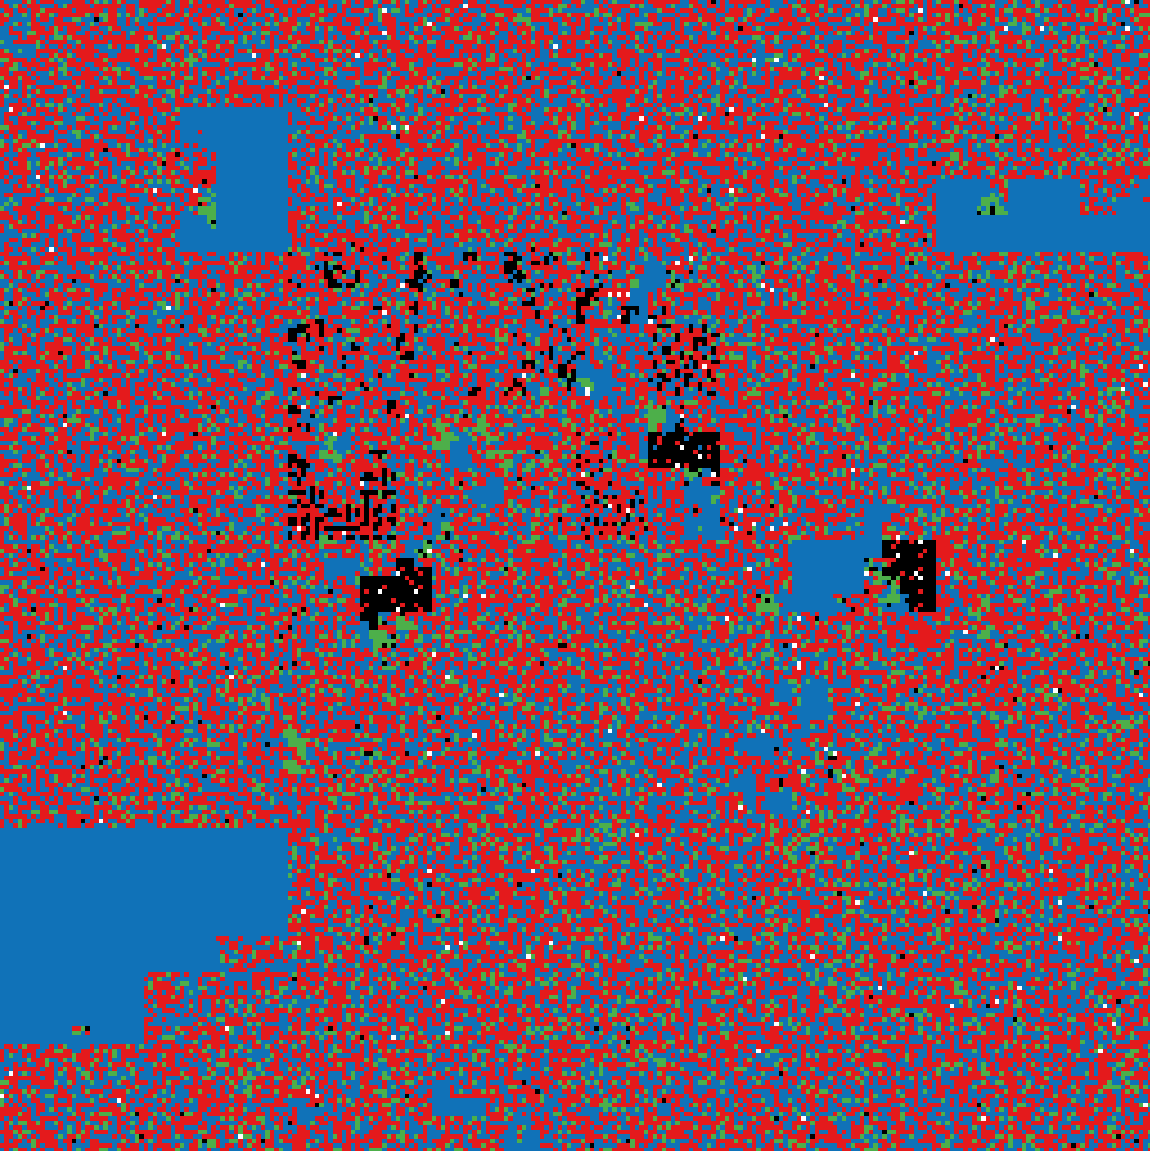
\includegraphics[height=5cm]{imgs/crowdstrike.png}
        \centering
        \caption{Part of the file visualisation}
        \label{fig:subim2}
    \end{subfigure}
    \centering
    \caption{Visualisation of file - feasible for every file.
    For such data, an analysis similar to image recognition techniques can be performed}
    \label{fig:image2}
\end{figure}
\FloatBarrier


\subsection{Parallel hybrid systems}\label{subsec:parallel-hybrid-systems}

In the paper \say{Is machine learning cybersecurity's silver bullet?} ESET's experts sort training data into three groups - malicious, clean and potentially unwanted.
They recommend not to use algorithm own output data as inputs, because any further errors are reinforced and multiplied, as the same incorrect result enters a~loop and creates more false positives or misses of malicious items~\cite{eset_machine_learning}.
In the next chapter ESET points out how crucial it is to achieve an equilibrium of sufficient protection from malicious items and false positives minimised to a~manageable level.
Finally, in the chapter \textit{Machine learning by ESET - The road to augur} authors let us take a~look under the hood of their ML engine called Augur.
For malicious file detection they are using two branches:
\begin{enumerate*}[label=(\roman*)]
    \item sandbox analysis followed by advanced memory analysis and behavioural features extraction (these features are later used to train ML models),
    \item ML-based branch.
\end{enumerate*}
ML-based branch consists of two methodologies:
\begin{enumerate*}[label=(\roman*)]
    \item neural networks, specifically deep learning and long short-term memory (LSTM),

    \item consolidated output of six classification algorithms.
\end{enumerate*}
While consolidating output of those six classification algorithms, two modes (setups) are used.
The first one is used for security critical environments, making algorithm more likely to mark file as malicious if most of the previous algorithms vote it as such.
The other setup is more conservative - labelling a~sample clean if at least one algorithm comes to such conclusion.

\begin{figure}[htb]
    \centering
    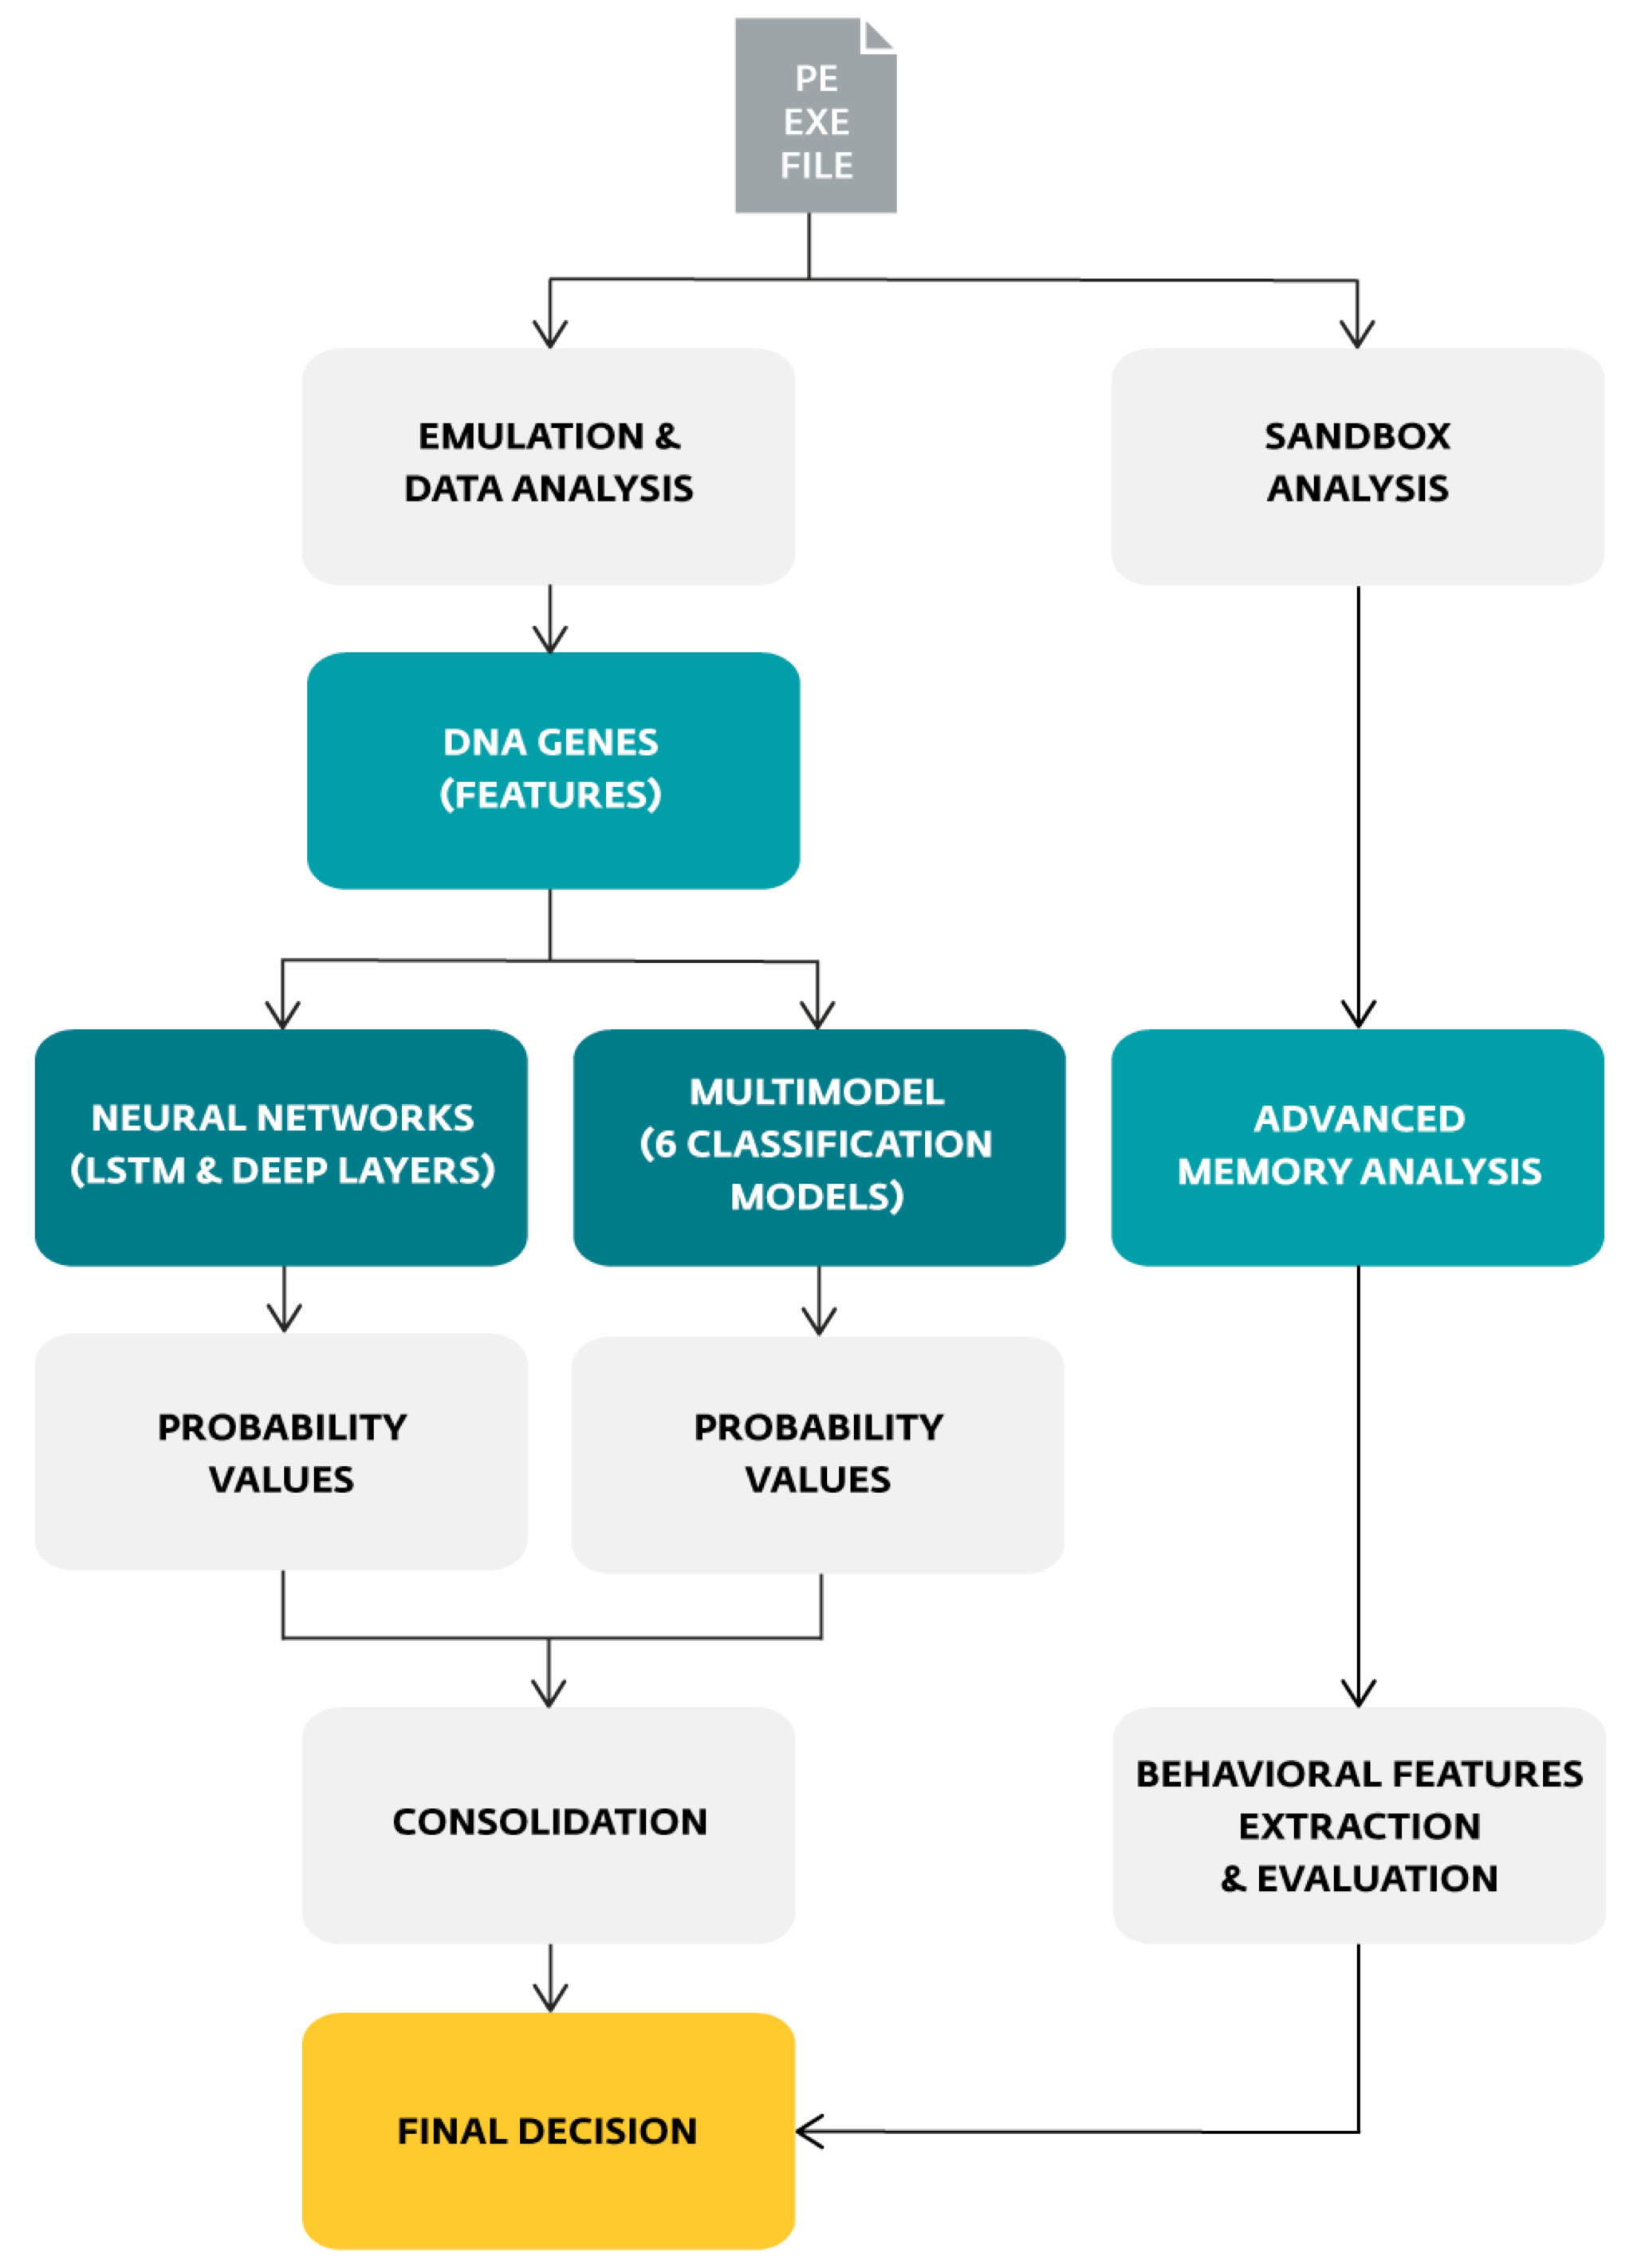
\includegraphics[width=0.5\textwidth]{imgs/eset_augur.png}
    \caption{Augur classification model~\cite{eset_machine_learning}}
    \label{fig:sim1}
\end{figure}
\FloatBarrier

\subsection{Serial hybrid systems}\label{subsec:serial-hybrid-systems}

\textit{Kaspersky Lab} identify an average of \num{360000} new items of malware every day - approximatelly \num{131400000} new threats per year~\cite{whitepaper:kaspersky_next_generation}.
Those security breaches result in direct financial losses, loss of business reputation or financial and legal penalties imposed by regulators.
\textit{Kaspersky} provide multi-layer solution consisting of:

\begin{enumerate}[label=(\roman*)]
    \item exposure prevention (network filtering),
    \item pre-execution detection based on machine learning,
    \item runtime control proactively looking out for suspicious behavior of devices in the network (behavioral analysis based on ML),
    \item automated response such as \textit{automatic rollback} to help restore systems to their pre-attack state, system disinfection techniques or Incident of Compromise (IoC) scanning~\cite{whitepaper:kaspersky_next_generation}.
\end{enumerate}

Locality-sensitive hashes (LSH) are Kaspersky's solution for malware detection, with ML system used for difficult to detect hashing regions~\cite{whitepaper:kaspersky_machine_learning}.
LSH's goal is to create a~reliable fingerprint - a~set of features -  of a~malicious file that could be checked instantaneously~\cite{whitepaper:kaspersky_machine_learning}.
This type of hash function maps very similar files to the same hash values - similar files maps to nearby surroundings.
A group of files with a~similar hash mapping value is called a~hash bucket~\cite{whitepaper:kaspersky_machine_learning}.
Those buckets can be either simple - containing only one type of objects (malware or benign), or hard - containing malware and benign samples.
Features are extracted from items in hard regions, to undergo ML classifiaction.
Various types of models are pre-trained with human annotated data.
Which model is selected for classification of items in region depends on several factors - extractable features, type of objects, etc.

\begin{figure}[htb]
    \centering
    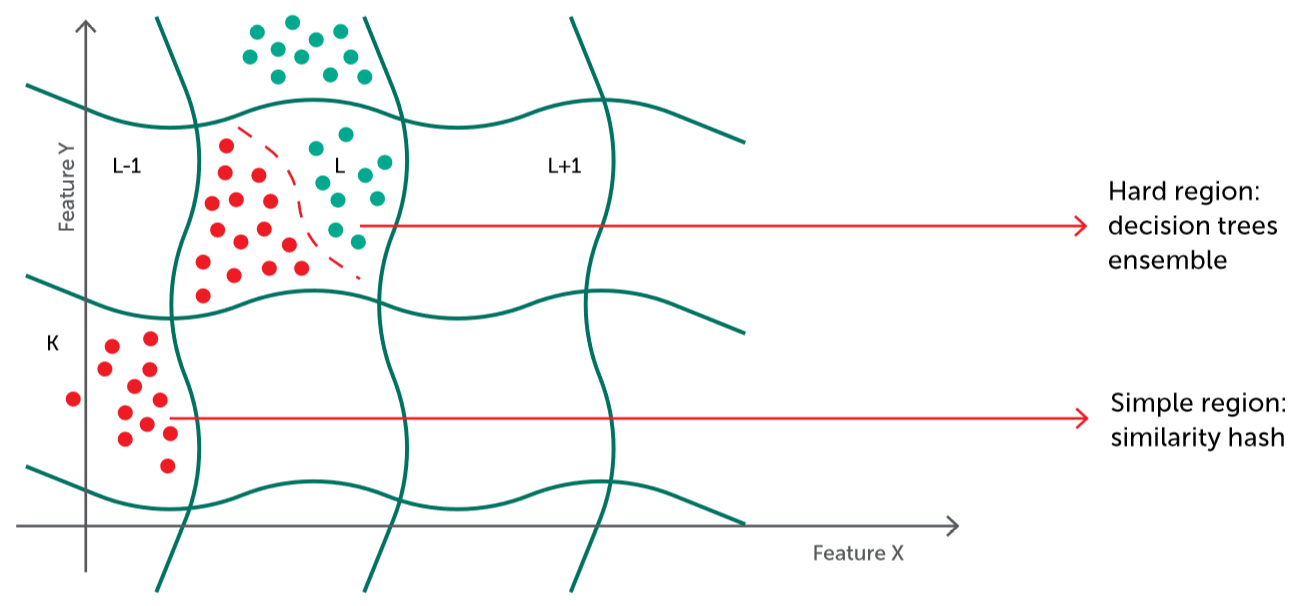
\includegraphics[width=0.9\textwidth]{imgs/kaspersky_regions.png}
    \caption{Segmentation of object space~\cite{whitepaper:kaspersky_machine_learning}}
    \label{fig:kaspersky_regions}
\end{figure}
\FloatBarrier

\subsection{Settlement}\label{subsec:settlement}

Circumstances show that although ML-based detection is adequately effective, it needs to be part of a~comprehensive solution to address complex security intrusions.
At the same time, security companies agree there is no guarantee that classifier can correctly identify all the new samples it encounters, therefore human verification is still needed.

\section{AI as target of attacks}\label{sec:ai-as-target-of-attacks}

AI algorithms faces severe security risks which can result in loss of confidence in the government or specific company, not to mention personal safety endanger or property loss.
According to the Huawei, there are five security challenges AI system design must overcome~\cite{huawei_security}.
Those five challenges are software and hardware security, data integrity, model confidentiality, model robustness and data privacy.

Firstly, application code and models themselves has to be reliable.
There is need for programming languages as well as for processors and GPUs to guarantee memory and thread safety.
Since january 2018 vulnerabilities related to modern CPUs fundamental attribute - speculative execution - became well known by names Spetre (CVE-2017-5753 and CVE-2017-5715), Meltdown (CVE-2017-5754), Foreshadow (CVE-2018-3615) or Spoiler (without \acrshort{cve} number so far).
Without solid solutions to mitigate consequences of those issues, attackers may implant backdoors into models to exploit data and construct sophisticated attacks to bring decision models into disrepute.
Moreover those attacks are due to limited explainability of AI models difficult to discover.

Second topic relate to data integrity.
There is serious concern that attackers can inject data while a~model is in the training stage to alter the inference capability or add disturbance into the input samples to change model's interpretation and distort result.

Third challenge involve fear of possible \say{hijacking} of model through its reconstruction, where data are captured by analyzing large numbers of input and output queries.
The fourth one points out insufficient model robustness, originating in training data, which are not good intepretation of real-world data or does not cover all possible edge cases.
Those aspects lead to model incompetency to provide trustworthy decisions.

Last risk appertain to data privacy and data leakage through repeated request to obtain users’ private information (in scenarios where model is actually trained on the data provided by users).
Research from 2013 shows, that using Facebook likes can be used to predict users intimate traits, that are not directly observable in the data.
By using ML algorithm you can predict intimate traits like sexual orientation, IQ or drug abuse~\cite{Kosinski5802}.
This research focused on Facebook likes, although similar research could be done using other kinds of digital footprints, like Spotify playlist, fragments of your Google searches and so on.
Possible leakage of data with analogous properties would have serious consequences.

Defending AI systems can become very challenging task.
All kinds of methods take an advantage of ML systems vulnerabilities.
In order to provide failsafe, data security and high availability guarantees, software architects has to construct system consisting of defense layers for known attacks (which are going to be discussed in the following sections), techniques (e.g.\ model verification mechanism or explainability of both data and model) for enhancing model robustness and procedures to ensure business security such as model isolation, application redundancy and training data consistency.

\subsection{Evasion}\label{subsec:evasion}

In security-sensitive applications, samples can be actively manipulated by an profound adversary to confound learning.
With the goal to avoid detection, spam emails are often modified by obfuscating common spam words or inserting words associated with legitimate emails~\cite{arxiv:evasion_attack}.
Such activity is called the evasion attack and can be induced either by modifying samples in form of virtual data (e.g.\ text, audio recording etc.) or by altering real world objects (ammending traffic signs or inducing noise signal).
To generate adversarial samples, attackers need to obtain AI model parameters.

In the paper presented by Papernot et al. is proposed technique for generating those examples without knowing exact parameters~\cite{arxiv:transferability_in_ml}.
They found that data which deceives one model can deceive another model as long as the training data of those two are the same.
This so called transferability is used to launch black-box attacks without knowing parameters of the target model.
Training data for substitute model are aquired by querying target model several times.
After training phase of the substitute, this model can be used to generate adversarial samples, which can be used to deceive the original model.
Papernots team archieved admirable results by mischeiving commercial machine learning classification systems from Amazon and Google with approximatelly 96\% and 89\% success rate respectively, using only 800 queries of the victim model.
This demonstration shows that current ML approaches are in general vulnerable to methodical black-box attacks regardless of their structure.

There are several ways to protect models against evasion attack.
The first approach is improve model robustness either by \textbf{network distillation} or \textbf{adversarial training}.

\textbf{Network distillation} is approach used as defense for \textit{deep neural networks}.
In principle, one DNN is linked together with the second (executive) DNN in a~chain.
The classification result from the supplementary DNN is used as training input to the other one.
This leads to the transfer of knowledge, reducing sensitivity to adversarial samples and improving the robustness of a~model - reducing the success rate of specific attacks such as \textit{Maximal Jacobian-based Saliency Map Attack}~\cite{arxiv:jacobian_attack}.

\textbf{Adversarial training} is arguably the simplest method and should be used to train every production-ready model.
If model architects have some \textit{a priori} knowledge about possible patterns of adversarial samples, they should use that information to generate some samples and use them to train the model~\cite{huawei_security}.
Training and possible retraining - after obtaining new information about malicious data - leads to more standardized more accurate and robust model~\cite{huawei_security}.

Other option is to append additional component to capture and therefore filter out malicious input sample before it gets into inference stage - \textbf{adversarial sample detection}.
Simple deterministic detector could be a~deterministic comparer having some type of \textit{distance} as a~criterion.
Detectors vary greatly - forming a~group of independent models worth exploring in other papers.
% possibility to write more about detectors - the detection model may extract related information at each layer of the original model to perform detection based on the extracted information

A deformed input samples does not effect normal classification function of a~model.
\textbf{Input reconstruction} works by deforming input samples to defend against evansion attack by adding noise, de-noising, or using an automatic encoder (a type of artificial neural network)~\cite{huawei_security}.

Last but not least method is \textbf{model verification}.
In general, verification is a~discipline of software engineering with goal to assure that software fully satisfies all the expected requirements.
Specifically, to verify model means producing a~compelling argument that the system will not misbehave under a~very broad range of circumstances~\cite{blog:model_verification_and_testing}.
To verify ML model a~set of legal inputs (similar to test set) has to be defined and verification techniques that guarantee the correctness of the machine learning predictions has to be designed.
Simultaneously the verification method has to consider the generalizing capabilities of a~model and varying properties of new inputs.
Because of those reasons, creating proper verification technique is not an easy task and could be researched as a~separate subject.

\subsection{Poisoning}\label{subsec:poisoning}

Data poisoning is a~class of attacks on machine learning where an adversary alters a~fraction of the training data in order to impair the intended function of the system.
Objective can be to degrade the overall accuracy of the trained classifier, escaping security detection or to favor one product over the another.
ML systems are usually retrained after deployment to adapt to changes in input distribution, so data poisoning represents serious danger.

Even though many papers focuses on this topic, presents diverse types of attacks and generally agrees that even a~small number of malicious training samples are needed to significantly affect the accuracy of models, majority aims their attention at offline learning - not so much on semi-online and online learning.
While semi-online mode means that system is learning from data stream but attacker cannot obtain classifiers objective until the end of training, online training means that both the training process and the evaluation of the objective are streamed - example of such system is stock market predicting model.
In the article called \say{Data Poisoning Attacks against Online Learning} researches propose several attack types and feasible defense setups for semi-online and online learning~\cite{arxiv:data_poisoning_online_learning}.
Performed experiments show that semi-online setting is more vulnerable than the fully-online setting.
In the end researchers recommend the use of online methods where classifier does not depends on a~just few input samples, so these methods would be less vulnerable to adversarial attacks.

One posibility to protect system against poisoning attack is \textbf{training data filtering}.
Detecting malicious samples and following purification of training data sets is not a~trivial task.
In paper from 2016 the researchers presented method called \say{Curie} for detecting poisonous samples in the dataset~\cite{arxiv:curie}.
This method works by working in (feature + label) space to filter out malicious samples.
Curie is an unsupervised method and an attacker would have to use evasion attacks to pass through Curie.
This means that the attacker would have to inject data that works both for evasion attack and poison attack.
Such attack would be very complicated to construct.

\textbf{Regression analysis} methods such as linear and ordinary least squares regression are ideal to detect noise and abnormalities in the data sets.
Thanks to relative directness presents those methods easy way to fight back data poisoning attack.

\textbf{Ensemble analysis} points out that usage of multiple sub-models - each one of them trained with different training data set - reduces probability of system being affected by poisoning attacks greatly.

\subsection{Backdoor}\label{subsec:backdoor}

Backdoor is in some respects similar to the poisoning attack.
Although in this case, attacker is not targeting overall shift in decision inference or accuracy - the model behaves as it should on normal conditions, but on a~specific input the output is controlled by adversary, causing malicious behavior when triggered.
Corrupting the model so the attack would be feasible can be challenging.
Option is to implant some specific neuron into the neural network or to inject carefully crafted samples into the training set.
This specific neuron would be called \say{neural trojan}.
In general, backdoor is a~malicious functionality embedded into the system.
The Trojan could have been embedded in the topology, the hardware implementation, or as additional circuitry.

There are againg several ways to mitigate such attack.
There is always possibility to try to detect input anomalies or to re-train model (supervised) with legitimate data only, hoping that the Trojans contained in the weights of neural network may be overwritten during the re-training process - requiring the NN to be reconfigurable~\cite{arxiv:neural_trojans}.
\textbf{Input pre-processing} aims to prevent the illegitimate inputs from triggering the Neural Trojans by using autoencoder~\cite{arxiv:neural_trojans}.

\textbf{Model pruning} is a~popular method for compressing a~neural network while keeping normal functions~\cite{arxiv:pruning_nn,arxiv:fine_pruning_nn}.
In addition, this method can be used as a~defense mechanism against backdoor attack by possibility of cutting off the \say{neural Trojan}.

\subsection{Model Extraction}\label{subsec:model-extraction}

As mentioned in section~\ref{subsec:poisoning} ML models are prone to extraction attack - especially those with public \acrshort{api} such as \textit{Google Cloud APIs}, \textit{Microsoft Cognitive Service} or \textit{Amazon Machine Learning}.
Via analysising input, output and other information about the model, its parameters, training data and structure can be speculated.
Those data can be latter used for black-box evansion attack, or just to steal the intellectual propperty the API and model itselves represents.
More information about this topic can be found in the paper from 2016, \say{Stealing Machine Learning Models via Prediction APIs}~\cite{usenix:stealing_models}.

\textbf{Model watermarking} embrace the risk of backdoor attack and makes it its advantage.
By embeding special neurons, model owners are able to check whether the model was stolen (copied) or not.
The disadvantage of this method is obvoius - it is prone to model pruning.

\subsection{System security}\label{subsec:system-security}

Previous examples of attacks on ML systems and possible defences apply only to specific scenarios.
Despite of possibility to combine multiple of these method/technologies in parallel or serially, it is not possible to completely defend against all attacks~\cite{huawei_security}.
Therefore it is necessary to prevent possibility of exposure by strengthening model architecture or by supervising and administrating training dataset to mitigate the posibility of data contamination~\cite{chio2018machine}.
Such incident would lead to users having a~cautious distrust of models reasoning.

Before model deployment, the system should be black-box and white-box tested in order to get some qualitative report about system security~\cite{huawei_security}.
Results from such testing could be refered as \textbf{model detectability} - from system theory a~system is detectable if all unstable states are observable - in such manner testers check if and how can be system's weaknesses abused.

In the section~\ref{subsec:evasion} the principle of \textbf{model verifiability} was already mentioned.
Unfortunatelly, for some ML models can be really hard to denote all edge cases.
It may be possible to restrict an input range or to apply a~saturation function in some cases, but due to complexity and variability of input data, it is not usually viable solution.

It may be difficult to fully interpret models inference process and it is not a~functional requirement to be able to do so, for many production systems.
On the other hand, there are dozens of solutions, which would benefit greatly from solution which would provide a~credible explanation for model inference process.
There are handful of solutions introducing \textbf{model explainability} to ML and there are overall three categories of possible implementations.
Latest literature uses phrase \textbf{Explainable AI (XAI)} to capture the essence of the problem.

\begin{table}
    \centering

    \begin{tabular}{llll}
        \toprule
        Algorithm & Linear & Monotone & Task \\
        \midrule
        Linear regression & Yes & Yes & regression \\
        Logistic regression & No & Yes & classification \\
        Decision trees & No & Some & classification \& regression \\
        RuleFit & Yes & No & classification \& regression \\
        Naive Bayes & No & Yes & classification \\
        K-nearest neighbors & No & No & classification \& regression \\
        \bottomrule
    \end{tabular}

    \caption{Explainable algorithms~\cite{webbook:interpretable_machine_learning} - model is \textbf{linear} if the association between features and target is modelled linearly; \textbf{monotonicity} refers to model's ability to ensure that the relationship between a~feature and the target outcome always goes in the same direction over the entire range of the feature, therefore an increase in the feature value leads either to always increase or always decrease in the target outcome}
    \label{table:explainable-algorithms}
\end{table}
\FloatBarrier

\begin{enumerate}
    \item \textbf{Explainable data}
    As Huawei in its paper mentions, if several representative characteristics can be found at data sets and those features are carefully selected, then a~some models can be meaningfully interpretted~\cite{huawei_security}.
    Of course, data set are not usually simple enough to make such analysis.
    Moreover, AI model can grow in complexity and even with understandable data and features in the beggining, there is no guarantee that result is intereprettable in the end.

    \item \textbf{Explainable model}
    Some of the ML models (either for classification or regression) are interprettable naturaly.
    Their typical properties are \textit{linearity}, \textit{monotonicity} and \textit{interaction features} - possibility to manually add non-linearity into the model.
    Those models are often way too simplistic for real-world applications, but for an idea those algorithms are sumarized in the table~\ref{table:explainable-algorithms}.

    \item \textbf{Explainability analysis}
    The last possibility is to analyze relation between input and output with (or without any) some knowledge about the classifier itselves.
    This solution is discussed in more detail in section~\ref{sec:explainer}.
\end{enumerate}

Finally there are security mechanisms based on business requirements~\cite{huawei_security}.
While AI model distribution, the engineers has to ensure architecture and deployment robustness.

\begin{enumerate}
    \item \textbf{Detection:} In some cases it is important to continuously monitor and scan for pottential attack signatures to estimate current risk level~\cite{huawei_security}.
    In case of high risk level, the steps are taken to ensure system and data safety.

    \item \textbf{Failsafe:} Failsafe is a~system design feature providing solution to counteract the effect of failure in order to couse the minimal damage to its surroundings.
    In AI systems, the failsafe mechanism can work by setting up a~certainty threshold.
    When output certainty is lower then threshold, the system can either use recovery procedures, redundant system (e.g.\ rule-based) or enter the manual processing~\cite{huawei_security}.

    \item \textbf{Isolation:} Isolation is very basic mechanism to improve security.
    Functional modules has to be separeted and their connection channels should provide mechanism to verify information validity and reliability.

    \item \textbf{Redundancy:} In a~security and infrastructure critical applications is indispensable to ensure system high-availability and robust decision inference process.
    A~multi-model architecture can reduce the possibility of the system being compromised by a~single attack, improving the robustness of the entire system~\cite{huawei_security}.

\end{enumerate}

\subsection{Data sets security}\label{subsec:data-sets-security}

In addition to model and architecture security mechanism, we have to consider security of data sets.
Data often contains personal information of users - so called \textit{sensitive attributes}.
Such information can be in a~form of personal identifiers or quasi-identifiers.
\textit{Personal identifier} is an unique information that identifies a~user - a~birth number, bank account number and other types of personal IDs.
\textit{Quasi-identifiers} are characteristics which needs to be used in combination with others to identify an entity - examples are gender, postal code, age or nationality.

To prevent data stealing and following re-identification of users, several models exists to protect personal information of individuals in dataset.
Those privacy models are \textbf{optimal k-anonymity}, \textbf{l-diversity}, \textbf{t-closeness} and \textbf{differential privacy}.
Three general types of attack to datasets exists:
\begin{enumerate*}[label=(\roman*)]
    \item \label{itm:reident} re-identifying an individual,
    \item \label{itm:query} query whether an individual is a~member of a~dataset,
    \item \label{itm:linking} linking an individual to a~sensitive attribute.
\end{enumerate*}

\textbf{Optimal k-anonymity} protects against both cases~\ref{itm:reident} and~\ref{itm:query} by transforming quasi-identifiers so that at least \( k - 1 \) members of set are indistinguishable from each other - group based anonymization.
Identifiers are transformed by suppression (needless attributes are replaced with \textit{dummy} values) and generalization (individual values of attributes are replaced with a~broader category - e.g.\ specific age can be replaced by a~range).
As \( k \) increases risk of data exploit reduces, on the other hand data quality decreases - we are talking about a~\textit{privacy-utility} tradeoff.
Moreover, the \( k \) is limit - in order for this method to work if \( k \) is set to \( k \triangleq 10 \) then any group must contain at least \( 10 \) individuals.
The first drawback of k-anonymity is vulnerability to \textit{homogeneity attack} which works on premise of data having sensitive value identical within a~set of \( k \) records - it is enough to find the group of records, the individual belongs to, if all of them have the same sensitive value.
Second drawback is the possibility of \textit{background knowledge attack} where attacker identifies associations among one or more quasi-identifiers and reduces the set of possible values for the sensitive attribute.

Both \textbf{l-diversity} and \textbf{t-closeness} are group based anonymization techniques building on a~concept of \textbf{optimal k-anonymity}.
In addition to \textbf{optimal k-anonymity}, \textbf{T-closeness} transforms quasi-identifiers such that each group is within a~distance \( t \) of the distribution of sensitive values for the entire dataset~\cite{web:privacy-models}.
The distance is measured as the cumulative absolute difference of the distributions, as \( t \) decreases both risk of sensitive attribute disclosure and data quality decreases.
Suppose that the sensitive attribute is salary.
Each group's frequency distribution of salary will be within a~distance \( t \) from the salary frequency distribution for the entire dataset~\cite{web:privacy-models}.

\textbf{Differential privacy} and its variants (epsilon, epsilon-delta) are statistical techniques aiming to protect data against \textit{differentiated attack}.
The model guarantees that even if someone has complete information about 99 of 100 people in a~data set, they still cannot deduce the sensitive information about the final person~\cite{web:differential-privacy}.
The mechanism works by adding random noise to the aggregate data, leaving only a~trend without possibility to figure out exact values in data (e.g.\ information that \( n\% \) of users prefer some product over another).

Some other techniques to keep dataset secure exist.
In some cases with very sensitive data, the data can be exported from database in a~form of already vectorized samples.
There is very little to be mined from data in such format.
On the other hand if data are not secured by any technology whatsoever, the risk rises.
A model may inadvertently or implicitly by design store some of its training data.
In this case careful analysis of the model may reveal sensitive information.
Solutions like \textbf{Private Aggregation of Teacher Ensembles} - PATE in shortcut - exist to adress this problem~\cite{huawei_security}.
\textit{PATE} works by segmenting training data into multiple sets, each for training an independent ML model~\cite{huawei_security}.
Those models are used to cooperatively train a~student model by voting.
It is assumed that an adversary cannot access teacher models - he can access only student model.
The student learns to predict an output chosen by voting among all of the teachers~\cite{huawei_security}.
The student is trained with public (not sensitive) data.
Model's privacy properties are indisputable - adversaries are not able to extract sensitive data with access to the student model only.

\section{The malicious use of ML in cybersecurity}\label{sec:the-malicious-use-of-ml-in-cybersecurity}

As machine learning provides protection against attackers, attackers themselves can exploit machine learning for malicious use.
The most obvious malicious use of ML is information gathering, which can be used for social engineering and personalized attacks (such as more sophisticated and believable phishing emails).
Another type of usage can be to break through Google's re\acrshort{captcha} which is test build specially to tell human and a~machine (a bot) apart~\cite{blog:breaking_captcha}.
ML methods can be certainly used with attacks mentioned in the section~\ref{sec:ai-as-target-of-attacks} - poisoning, model extraction or evasion attack as presented in paper by \textit{Weiwei Hu} and \textit{Ying Tan}, \say{Generating Adversarial Malware Examples for Black-Box Attacks Based on GAN} where authors describe how they built a~\textit{generative adversarial network (GAN)} based algorithm, that will be able to bypass ML detection protection system~\cite{arxiv:real_evasion}.

Nowadays, a~sophisticated ML supported malware imitating human attacker's behavior starts to appear.
The expert human adversary try to blend into their target environment as much as possible, in order to remain hidden.
To achieve \say{invisibility}, the attacker understands what normal behavior of the infected system looks like and adjusts his techniques accordingly.
It is possible for malware to acquire this contextual understanding and integrate into a~target environment autonomously.

All following techniques are just usages of user and process behavior analysis, but represents real threats and trends in malicious software development.
In the research white paper \say{The Next Paradigm Shift: AI-Driven Cyber-Attacks}, cybersecurity company \textit{Darktrace} presents three inovative attack scenarios, in which attackers used ML for more successfull infiltration.
Each threat covers different phase of the attack cycle - lateral movement, C\&C traffic and data exfiltration.

\begin{figure}[htb]
    \centering
    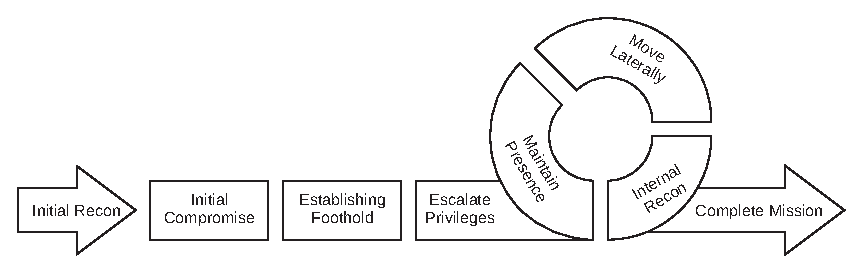
\includegraphics[width=0.9\textwidth]{imgs/attack-cycle.eps}
    \caption{Malware attack lifecycle~\cite{article:attack_lifecycle}}
    \label{fig:malware_attack_cycle}
\end{figure}
\FloatBarrier

\subsection{Trickbot: smart assault method selection}\label{subsec:trickbot:-smart-assault-method-selection}

First case represents a~modular malware \textit{Trickbot} - a~banking \textit{Trojan} type malware targeting Windows machines.
\textit{Trickbot} malware is being developed and improved for several years now (at least from 2016), and was extended by numerous additional capabilities, such as:

\begin{itemize}
    \item achieving persistence (through scheduled tasks),
    \item disabling Microsoft’s Windows Defender (built-in antivirus),
    \item gathering email addresses and sending out spam,
    \item collecting system and memory information, user accounts, lists of installed programs and services,
    \item fingerprinting browsers and capturing data from them (including passwords),
    \item steal passwords from Microsoft Outlook and FTP applications like WinSCP or Filezilla,
    \item spreading itself to other computers on the same network by exploiting SMB vulnerabilities with the EternalRomance exploit~\cite{web:trickbot}.
\end{itemize}

Besides SMB protocol exploits, \textit{Trickbot} is spread via email attachments, malicious URLs, Microsoft Word documents with macros and other malware like Emotet.
The stolen information is exfiltrated to C\&C servers and used to achieve continuous access to infected networks and to deliver ransomware - e.g.\ Ryuk, specialized in targeting enterprises.
Version of \textit{Trickbot} discovered by \textit{Darktrace} installed program called \textbf{Empire}, the PowerShell post-exploitation agent.
This allows the attackers to conduct manual intrusions, for high-value targets.

At least two potential and dangerous ML-based improvements of Trickbot exist.
Malware could autonomously utilize multiple payloads for monetization – for example stealing banking details and locking machines for ransom.
This functionality is already available, but its modularity encourage to use ML and intelligently choose which payload will yield the highest profit based on the context of the environment and infected machine.
Second improvement is to analyse target environment and select best self-propagation process.
Ability to choose lateral movement techniques accordingly makes communication with C\&C server unnecessary (until need to send information), making attack stealthier, more difficult to detect and therefore more dangerous.

\subsection{Intelligent evasion}\label{subsec:intelligent-evasion}

Next case shows malware ability to analyze its environment to remain hidden for longer periods of time.
At a~utility company, the malware used a~variety of stealth tactics and obfuscation to stay hidden.
Malware was downloaded to the device from the Amazon S3 cloud platform - attacks exploiting Software-as-a-Service (SaaS) like Google Apps Script to deliver malware via URLs are quite common.

The malware showed ability of blending into the environment - utilizing its own self-signed SSL certificate for windowsupdate.microsoft.com and made HTTP(S) requests to an attacker-controlled IP address utilizing the fake Windows certificate.
In order to remain unseen, the communication took place over the \textit{well-known ports} like 443 for Hypertext Transfer Protocol over TLS/SSL (HTTPS) and 80 for Hypertext Transfer Protocol (HTTP), therefore blending in with regular network traffic.

According to Open Source Intelligence (OSINT) it is expected, that most malware will be improved with ML-based capability to blend into its environment, without need to be highly targeted.
This skill will come in forms of establishing C2 channels during regular business hours, communication over the well-known ports, using domain names for C2 communication and data exfiltration that closely resemble the target’s own domain or company name or domain fronting for popular content delivery networks.

Malware will learn about its environment via user and process bahavior analysis to gain an understanding of what communication will be most effective in the target’s network.
